% !TEX root = ../main.tex
%
% 第五章 作品测试与分析
% 每个 subsection 对应 chapter5/ 目录下的独立文件，方便维护和编译定位。
%
\section{作品测试与分析}

本章对 FoodShield 系统进行全面测试与分析，验证系统功能完整性、安全机制有效性、日志完整性检测能力、访问控制边界以及关键路径性能。测试内容与第三章威胁模型中定义的各类攻击场景严格对应，旨在证明系统设计中的安全目标在实际实现中得到有效落地。

% !TEX root = ../../main.tex
\subsection{测试环境}

FoodShield 系统的测试环境配置如表~\ref{tab:test_env}所示。所有测试均基于 Flask 内置测试客户端完成，使用独立的临时数据库，不修改演示数据库，确保测试结果的可复现性和数据隔离性。

\begin{table}[H]
\centering
\caption{测试环境配置}
\label{tab:test_env}
\begin{tabular}{ll}
\hline
\textbf{项目} & \textbf{配置} \\
\hline
操作系统 & Arch Linux（WSL2，Kernel 6.18.33.1） \\
CPU & Intel i5-13420H（WSL2 分配 2 核 4 线程，2.611\,GHz） \\
内存 & 7.8\,GiB \\
Python 版本 & 3.13 \\
国密算法库 & gmssl \\
数据库 & SQLite 3 \\
测试框架 & Flask test client（隔离数据库） \\
\hline
\end{tabular}
\end{table}

测试方法分三类：功能测试（正向调用各业务接口验证流程正确性）、安全测试（攻击演示脚本 \texttt{attack\_demo.py} 模拟各类威胁场景）、性能测试（基准脚本在不同数据规模下收集关键路径耗时）。

% !TEX root = ../../main.tex
\subsection{功能测试}

本节对 FoodShield 系统的核心功能进行正向测试，覆盖用户注册、PID 生成、口令认证、订单创建与 Token 生成、Token 验证、骑手接单、双向实时通信、消息加密存储、Merkle 快照生成、条件溯源和三端一致性验证等关键功能。测试结果如表~\ref{tab:func_test}所示，14 项测试全部通过。系统各端运行界面截图详见第四章 4.10 节。

\begin{table}[H]
\centering
\caption{功能测试用例与结果}
\label{tab:func_test}
\footnotesize
\setlength{\tabcolsep}{4pt}
\begin{tabular}{clllcc}
\hline
\textbf{编号} & \textbf{测试项} & \textbf{输入描述} & \textbf{预期结果} & \textbf{实际} & \textbf{结论} \\
\hline
F01 & 用户注册 & 用户名+密码+验证码 & 生成PID & 通过 & $\checkmark$ \\
F02 & PID生成 & 注册后自动 & 前端不展示 & 通过 & $\checkmark$ \\
F03 & 用户登录 & 用户名+密码 & SM3验证通过 & 通过 & $\checkmark$ \\
F04 & 创建订单 & 登录用户 & 生成orderID+Token & 通过 & $\checkmark$ \\
F05 & Token验证 & 合法Token & valid=true & 通过 & $\checkmark$ \\
F06 & Token过期 & 超时时间戳 & valid=false & 通过 & $\checkmark$ \\
F07 & 骑手注册 & 骑手信息 & 生成rider\_pid & 通过 & $\checkmark$ \\
F08 & 骑手接单列表 & 骑手登录 & 不展示PID & 通过 & $\checkmark$ \\
F09 & 骑手接单 & 骑手+orderID & 状态变更 & 通过 & $\checkmark$ \\
F10 & 实时通信 & 同订单房间 & 消息收发 & 通过 & $\checkmark$ \\
F11 & 加密存储 & 发送消息 & content为密文 & 通过 & $\checkmark$ \\
F12 & Merkle快照 & 管理员触发 & Root入审计日志 & 通过 & $\checkmark$ \\
F13 & 条件溯源 & 用户申请+审批 & 返回用户信息 & 通过 & $\checkmark$ \\
F14 & 三端一致性 & 管理员验证 & 三方Root一致 & 通过 & $\checkmark$ \\
\hline
\end{tabular}
\end{table}

其中，Token 生成采用$\mathrm{HMAC\text{-}SM3}(K_{\mathrm{order}}, \mathit{orderID} \| \mathrm{PID} \| \mathit{timestamp} \| \mathit{nonce})$，验证时后端从 session 获取 PID，不信任前端提交值。消息写入前经 SM4-CBC 加密（独立 IV），数据库存储$\mathrm{IV}+\mathrm{ciphertext}$。三端一致性验证比对管理员、用户和骑手各自上报的 Merkle Root，三者完全一致方判定通过。

% !TEX root = ../../main.tex
\subsection{安全性测试}

本节使用攻击演示脚本（\texttt{attack\_demo.py}）针对第三章定义的各类威胁场景进行安全测试。脚本包含 11 个场景（含 2 个正常操作基线），测试结果如表~\ref{tab:security_test}所示，完整运行输出如图~\ref{fig:attack_demo}所示。

\begin{table}[H]
\centering
\caption{安全性测试用例与结果}
\label{tab:security_test}
\small
\begin{tabularx}{\textwidth}{c l l X X c c}
\hline
\textbf{编号} & \textbf{攻击类型} & \textbf{威胁} & \textbf{攻击手段} & \textbf{预期防御} & \textbf{实际} & \textbf{结论} \\
\hline
S01 & 未登录创建订单 & T1 伪造 & 无登录态调用创建订单 & 401 拒绝 & 401 & ✓ \\
S02 & 伪造 Token & T2 伪造 & 修改 Token 末位字符 & valid=false & valid=false & ✓ \\
S03 & 跨用户越权 & T1 越权 & mallory 验证 alice 订单 & 403 拒绝 & 403 & ✓ \\
S04 & 未登录接单 & T1 伪造 & 无登录态调用接单 & 401 拒绝 & 401 & ✓ \\
S05 & 正常接单（基线） & — & 骑手首次接单 & 200 成功 & 200 & ✓ \\
S06 & 重复接单 & T6 滥用 & 同一骑手再次接单 & 400 拒绝 & 400 & ✓ \\
S07 & 管理员越权 & T6 越权 & 无登录态访问管理员接口 & 403+审计日志 & 403 & ✓ \\
S08 & 管理员登录（基线） & — & demo 账号登录 & 200 成功 & 200 & ✓ \\
S09 & hash-only 审计 & T7 隐私 & 管理员查看消息接口 & 无 content 字段 & 无 content & ✓ \\
S10 & 篡改检测 & T4 完整性 & 修改 DB 消息密文 & VERIFY\_FAIL & mismatch=1 & ✓ \\
S11 & 溯源滥用阻断 & T5 追责 & 调用明文关键词溯源 & 403 阻断 & 403 & ✓ \\
\hline
\end{tabularx}
\end{table}

\begin{figure}[H]
\centering
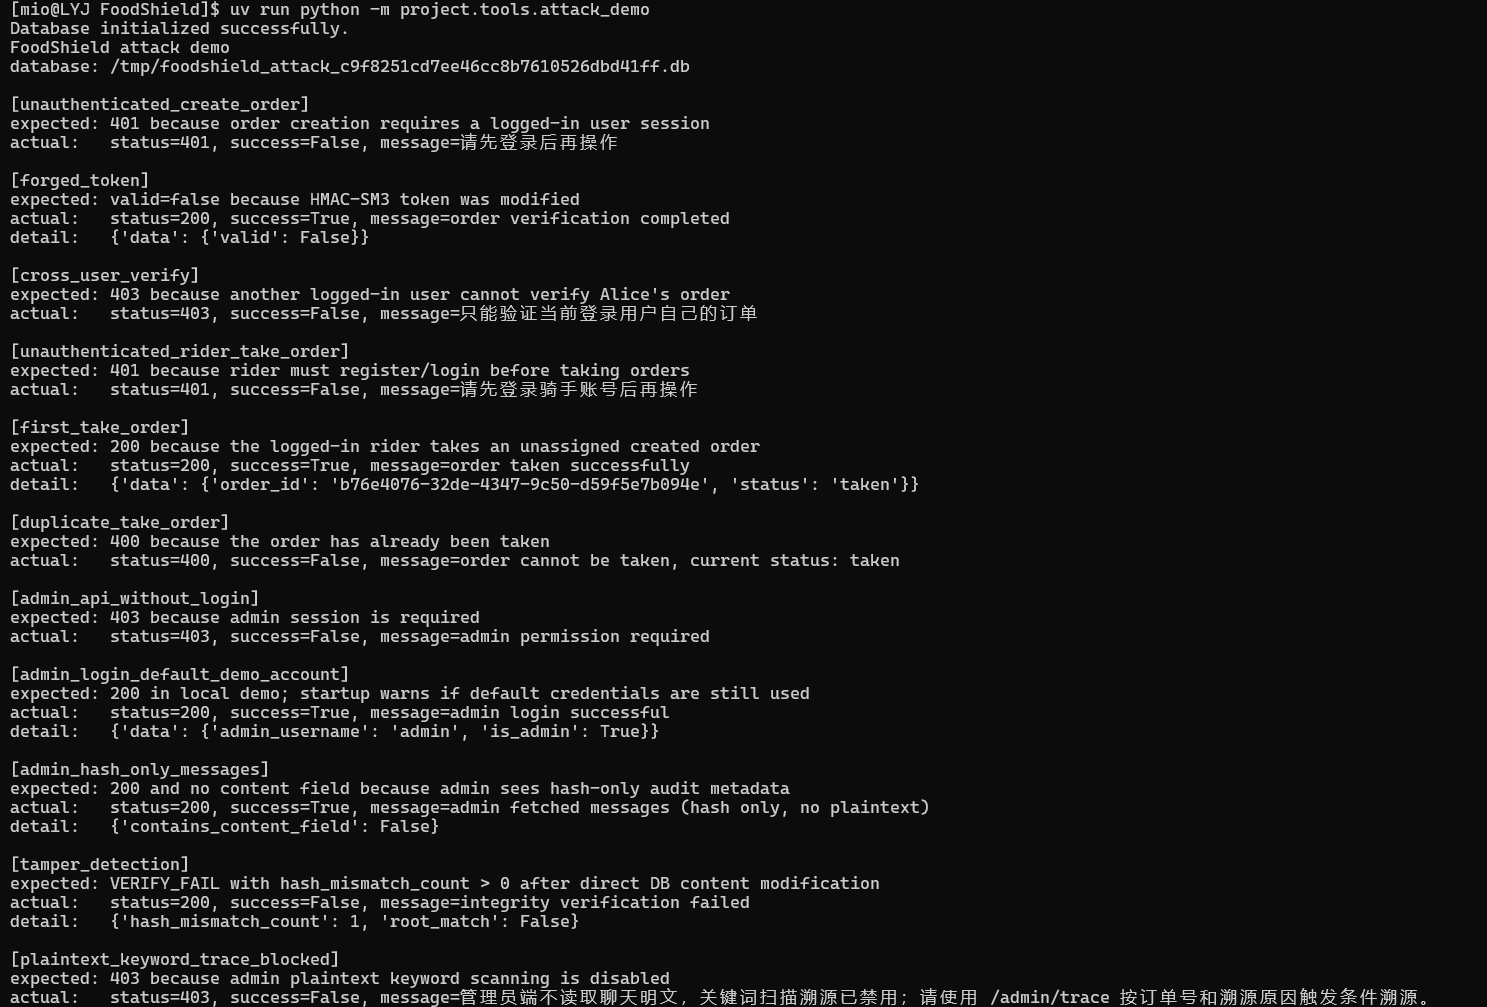
\includegraphics[width=0.95\textwidth]{content/chapter5/figure/attack_demo.png}
\caption{attack\_demo.py 运行输出（11 个场景全部通过）}
\label{fig:attack_demo}
\end{figure}

\textbf{S01--S02：身份与 Token 伪造}。无登录态请求被 \texttt{user\_required} 装饰器拦截返回 401；篡改 Token 末位后，\texttt{verify\_token} 重算 HMAC-SM3 发现不匹配，返回 \texttt{valid=false}，证明在未知$K_{\mathrm{order}}$下 Token 不可伪造。

\textbf{S03：跨用户越权}。后端从 session 获取当前用户 PID 与订单归属 PID 比对，不一致即返回 403，防止 Token 跨用户复用。

\textbf{S04--S06：骑手接单}。S04 验证未登录骑手被拒（401），S05 为基线（首次接单成功，状态 \texttt{created}$\to$\texttt{taken}），S06 验证重复接单被状态机拦截（400）。S05 的成功是 S06 拒绝的前提，两者共同证明接单状态约束有效。

\textbf{S07--S08：管理员访问}。S07 验证无管理员 session 时返回 403 并写入审计日志（action=\texttt{TRACE\_DENIED}），S08 为基线证明管理员认证流程正常。

\textbf{S09：hash-only 审计}。管理员消息接口返回数据仅含 \texttt{msg\_id}、\texttt{role}、\texttt{message\_hash} 和 \texttt{timestamp}，不含 \texttt{content} 字段，实现审计与隐私访问的接口级权限分离。

\textbf{S10--S11：完整性与溯源}。S10 验证篡改消息密文后完整性验证返回\texttt{VERIFY\_FAIL}（\texttt{hash\_mismatch\_count=1}，\texttt{root\_match=False}），详见 5.4 节。S11 验证管理员无法绕过审批流程直接扫描明文，溯源接口返回 403，溯源必须经完整性校验和审批双重门槛。

% !TEX root = ../../main.tex
\subsection{日志篡改检测测试}

本节验证 Merkle Tree 完整性机制对通信日志篡改的检测能力，覆盖修改密文、删除消息、插入伪造消息和顺序重排四种篡改类型。测试在数据库层面直接执行，模拟内部攻击者物理访问 SQLite 的场景。

首先建立正常通信场景：用户与骑手在同一订单房间发送多条消息，管理员生成 Merkle Root 快照。此时完整性验证返回 \texttt{VERIFY\_OK}，所有消息哈希一致，当前 Root 与快照 Root 匹配。

随后执行篡改：攻击者直接修改数据库中某条消息的加密内容字段。由于消息哈希绑定原始明文，修改密文后解密结果与原哈希不匹配。完整性验证返回 \texttt{VERIFY\_FAIL}，\texttt{hash\_mismatch\_count} $= 1$，\texttt{root\_match} $=$ \texttt{False}。该场景的运行输出见 5.3 节图~\ref{fig:attack_demo} 中 \texttt{[tamper\_detection]} 部分。四种篡改类型检测结果如表~\ref{tab:tamper_compare}所示。

\begin{table}[H]
\centering
\caption{篡改类型与检测结果}
\label{tab:tamper_compare}
\small
\begin{tabular}{llcc}
\hline
\textbf{篡改类型} & \textbf{Root 变化} & \textbf{mismatch\_count} & \textbf{验证结果} \\
\hline
修改消息密文 & Root 变化 & 1 & VERIFY\_FAIL \\
删除消息记录 & Root 变化 & 0 & VERIFY\_FAIL \\
插入伪造消息 & Root 变化 & 0 & VERIFY\_FAIL \\
消息顺序重排 & Root 变化 & 0 & VERIFY\_FAIL \\
\hline
\end{tabular}
\end{table}

其中"修改密文"已通过 attack\_demo 脚本 S10 项实际验证，其余三种基于 Merkle Tree 机制分析：删除、插入和重排虽不产生逐条哈希不匹配，但均改变 Merkle Tree 结构导致 Root 值变化。

综合测试结论：（1）内容篡改可精确定位——系统不仅检测到 Root 不匹配，还能报告 \texttt{stored\_hash} 与 \texttt{expected\_hash} 的差异条目；（2）结构篡改可全局检测——删除、插入和重排通过 Root 比对检测到完整性异常；（3）三端一致性增强——攻击者需同时篡改三方存储的 Root 才能伪造一致结果，单方面篡改必然被暴露。上述结论与第三章安全性分析一致：SM3 抗碰撞性（碰撞复杂度 $2^{128}$）保证字段修改后哈希以压倒性概率改变，Merkle Tree 级联特性保证叶子变化传导至 Root。

% !TEX root = ../../main.tex
\subsection{越权访问测试}

本节验证系统三层访问控制边界的严格执行能力。部分场景与 5.3 节安全测试重叠（S03 跨用户越权、S07 管理员越权），此处补充骑手越权和审计日志细节。

\textbf{用户越权}：用户 alice 尝试查看非本人订单的消息历史，后端校验 session 中 \texttt{user\_id} 与订单归属不一致，返回 403。

\textbf{骑手越权}：非接单骑手尝试进入订单房间发送消息或查看通信记录，后端校验 \texttt{rider\_id} 不一致，返回 403。

\textbf{管理员越权}：未登录用户访问管理员审计接口，全部返回 403 并写入审计日志，如表~\ref{tab:access_audit}所示。

\begin{table}[H]
\centering
\caption{越权访问审计日志记录}
\label{tab:access_audit}
\small
\begin{tabularx}{\textwidth}{X c l l}
\hline
\textbf{接口路径} & \textbf{状态码} & \textbf{审计 action} & \textbf{拒绝原因} \\
\hline
\path{/admin/messages/{OID}} & 403 & TRACE\_DENIED & not\_admin \\
\path{/admin/audit_logs/{OID}} & 403 & TRACE\_DENIED & not\_admin \\
\path{/admin/verify/{OID}} & 403 & TRACE\_DENIED & not\_admin \\
\path{/admin/orders} & 403 & TRACE\_DENIED & not\_admin \\
\path{/admin/trace} (POST) & 403 & TRACE\_DENIED & not\_admin \\
\hline
\end{tabularx}
\end{table}

\textbf{溯源滥用阻断}：管理员未经审批尝试明文关键词扫描，系统返回 403 阻断。当前溯源流程为审批式——用户/骑手提交溯源申请，管理员审批后按订单号自动完成溯源，管理员不能绕过审批直接扫描明文。

三层访问控制与 PID 后端托管、hash-only 审计共同实现第三章定义的目标五（可追责性）和目标七（隐私最小化）。管理员越权操作的审计记录使管理员自身行为也处于可追踪视野中，防止"谁来审计审计者"的信任困境。

% !TEX root = ../../main.tex
\subsection{性能测试}

本节使用性能基准脚本对关键密码学操作和业务流程进行耗时测试。两组测试分别使用不同数据规模（第一组：10 用户、50 订单、1000 消息；第二组：20 用户、200 订单、6000 消息），结果如表~\ref{tab:perf_basic}所示，终端运行输出如图~\ref{fig:perf1}和图~\ref{fig:perf2}所示。

\begin{table}[H]
\centering
\caption{关键路径性能基准}
\label{tab:perf_basic}
\small
\setlength{\tabcolsep}{4pt}
\begin{tabular}{lrrrrrcrrrrr}
\hline
& \multicolumn{5}{c}{\textbf{第一组（50 订单，1000 消息）}} & & \multicolumn{5}{c}{\textbf{第二组（200 订单，6000 消息）}} \\
\cline{2-6} \cline{8-12}
\textbf{操作} & \textbf{avg} & \textbf{P95} & \textbf{max} & \textbf{N} & \textbf{单位} & & \textbf{avg} & \textbf{P95} & \textbf{max} & \textbf{N} & \textbf{单位} \\
\hline
Token 生成 & 1.199 & 1.488 & 1.862 & 50 & ms & & 1.181 & 1.421 & 1.888 & 200 & ms \\
Token 验证 & 1.133 & 1.374 & 1.683 & 50 & ms & & 1.130 & 1.379 & 4.007 & 200 & ms \\
SM4 加解密 & 0.547 & 0.607 & 1.641 & 1000 & ms & & 0.550 & 0.624 & 3.975 & 6000 & ms \\
消息写入+哈希 & 0.454 & 0.582 & 1.355 & 1000 & ms & & 0.461 & 0.577 & 4.242 & 6000 & ms \\
Merkle 快照 & 19.90 & 21.29 & 21.76 & 50 & ms & & 28.17 & 29.82 & 32.82 & 200 & ms \\
完整性验证 & 37.62 & 39.09 & 40.69 & 50 & ms & & 54.48 & 57.02 & 61.09 & 200 & ms \\
\hline
\end{tabular}
\end{table}

\begin{figure}[H]
\centering
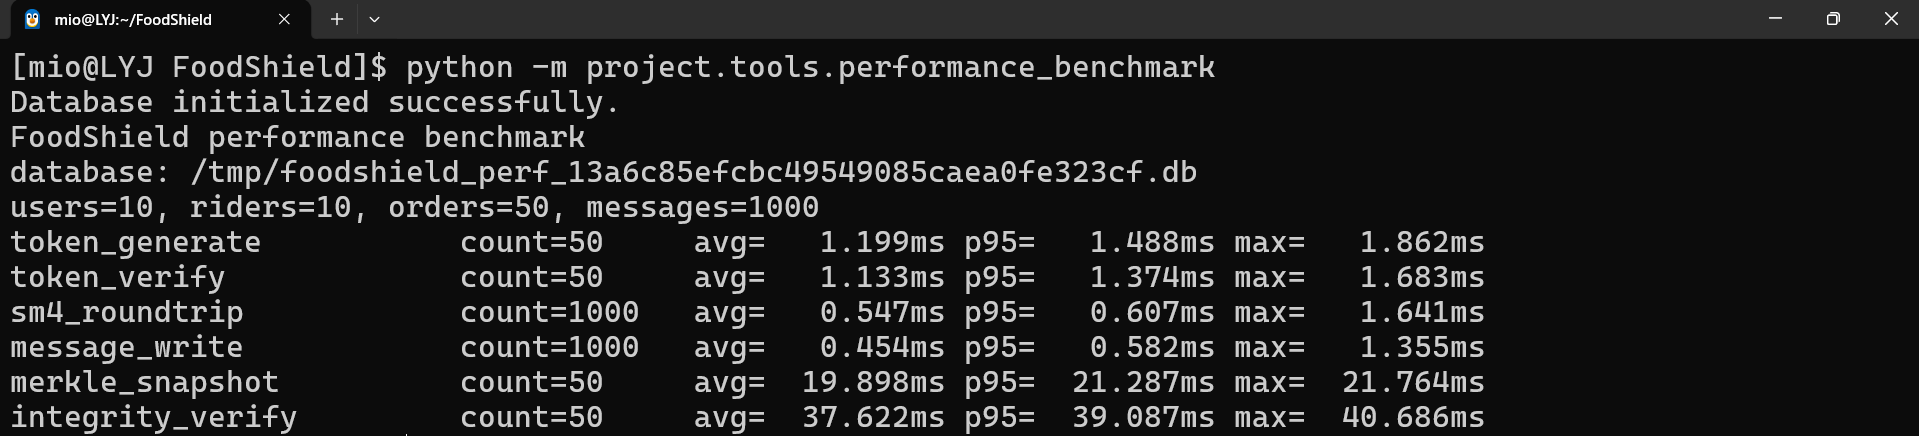
\includegraphics[width=0.95\textwidth]{content/chapter5/figure/perf.png}
\caption{第一组性能基准运行输出}
\label{fig:perf1}
\end{figure}

\begin{figure}[H]
\centering
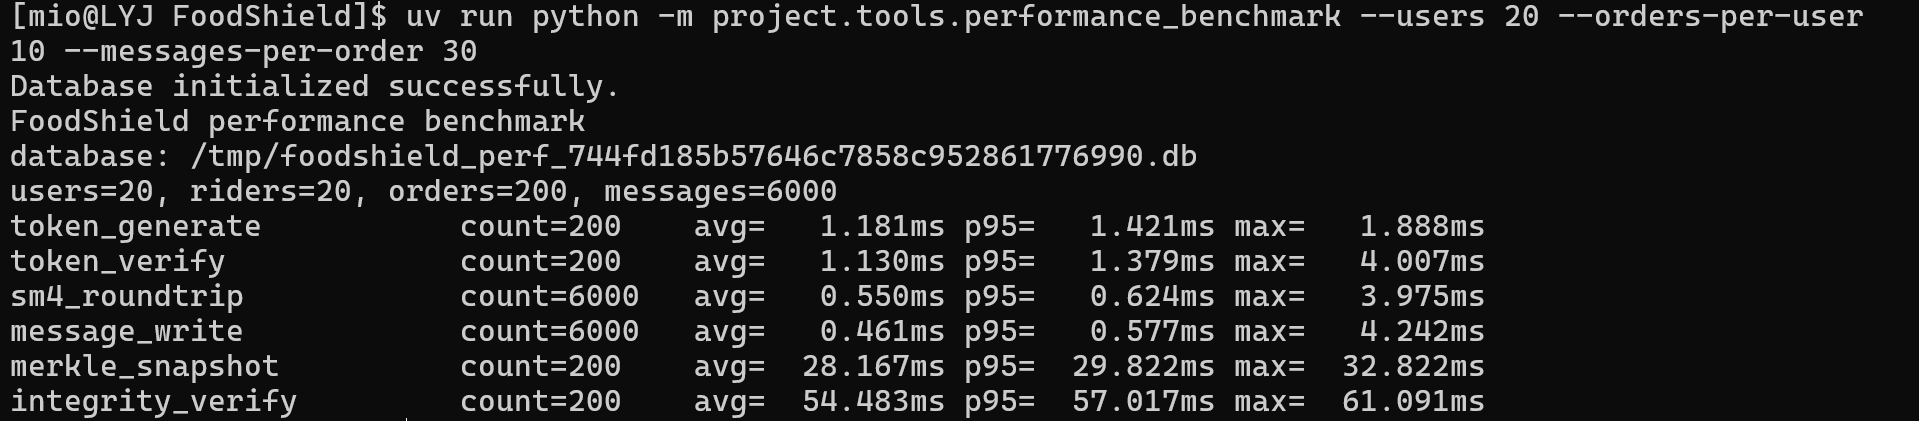
\includegraphics[width=0.95\textwidth]{content/chapter5/figure/perf2.png}
\caption{第二组性能基准运行输出}
\label{fig:perf2}
\end{figure}

\textbf{运行命令}：第一组 \texttt{python -m project.tools.performance\_benchmark}；第二组追加 \texttt{--users 20 --orders-per-user 10 --messages-per-order 30}。

\subsubsection*{性能分析}

\begin{enumerate}[label=\arabic*., leftmargin=2em]
\item \textbf{密码学操作耗时可控}：Token 生成与验证约 1.1--1.2\,ms，两组基本一致，说明 HMAC-SM3 耗时不受数据规模影响。SM4 加解密约 0.55\,ms，消息写入（含加密+哈希+SQLite INSERT）约 0.46\,ms，均满足实时通信要求。PID 生成同为 HMAC-SM3 操作，耗时与 Token 相当。

\item \textbf{Merkle 线性增长}：快照生成从 19.90\,ms（20 条/订单）增至 28.17\,ms（30 条/订单），每条消息约 0.94--0.99\,ms；完整性验证从 37.62\,ms 增至 54.48\,ms，每条约 1.82--1.88\,ms，均符合$O(n)$理论预期。

\item \textbf{瓶颈识别}：完整性验证是最耗时操作（需解密全部消息并重算哈希），但触发频率低（仅管理员主动验证或溯源前置校验时触发），不影响日常通信。日常关键路径（Token 验证 + SM4 加解密 + 消息写入）总耗时约 2\,ms。
\end{enumerate}

% !TEX root = ../../main.tex
\subsection{对比分析}

本节将 FoodShield 与现有外卖平台通信方案、普通 WebSocket 通信系统以及学术匿名通信方案进行安全特性对比，如表~\ref{tab:compare}所示。

\begin{table}[H]
\centering
\caption{FoodShield 与现有方案安全特性对比}
\label{tab:compare}
\footnotesize
\setlength{\tabcolsep}{3pt}
\begin{tabular}{lcccc}
\hline
\textbf{安全属性} & \textbf{FoodShield} & \textbf{美团/饿了么} & \textbf{普通WebSocket} & \textbf{群签名方案} \\
\hline
G1 匿名性 & PID强匿名 & 虚拟号码（弱） & 无匿名 & 签名匿名 \\
G2 认证性 & HMAC-SM3 & 无凭证认证 & 无认证 & 群签名认证 \\
G3 机密性 & SM4-CBC加密 & 传输加密+明文 & 传输加密+明文 & 加密（可选） \\
G4 完整性 & SM3+Merkle & 无验证 & 无验证 & 无Merkle \\
G5 可溯源 & 条件溯源 & 实名查询 & 不可溯源 & 群管理打开 \\
G6 抗滥用 & 验证码+限流 & 无机制 & 无机制 & 群成员管理 \\
G7 隐私最小化 & hash-only & 全量可见 & 全量可见 & 条件打开 \\
系统原型 & 已实现 & 商业运行 & 通用实现 & 仅理论 \\
\hline
\end{tabular}
\end{table}

\textbf{与美团/饿了么对比}：现有平台采用虚拟号码和脱敏显示，但存在三个不足：虚拟号码仅保护手机号，骑手仍可通过订单备注和地址推断用户习惯；管理员可无条件查看通信明文，缺乏权限分离；通信记录明文存储，无完整性验证。FoodShield 通过 PID（跨订单不可链接）、SM4 加密存储、hash-only 审计和 Merkle 完整性验证系统性改进了上述问题。

\textbf{与普通 WebSocket 对比}：普通 WebSocket 仅依赖传输层加密，攻击者获取订单号即可进入通信通道（无 Token 认证），管理员可查看全部明文，日志可被任意篡改。FoodShield 在通信层之上叠加了 Token 认证、PID 匿名、SM4 加密和 Merkle 验证，将普通即时通信升级为可认证、可审计的安全通信。

\textbf{与群签名方案对比}：群签名在理论上提供更强的匿名性（不可链接性），但存在三个实际限制：签名/验证涉及多次双线性映射运算，单次耗时数十毫秒，不适合高频低延迟的外卖通信；缺乏 Merkle 等完整性保护机制；未见针对外卖场景的系统原型。FoodShield 虽匿名性理论强度稍逊，但在计算效率、完整性和系统可用性方面更具优势。

\textbf{综合评价}：FoodShield 的核心差异化在于"可控匿名"模型——日常通信中对骑手和攻击者实现 PID 强匿名，同时在投诉驱动和审批约束下保留条件溯源能力。该模型介于"完全实名不可匿"与"完全匿名不可治"之间，在外卖订单通信场景中实现了匿名性、认证性、机密性、完整性、可溯源性和隐私最小化的多目标平衡。

